\documentclass[11pt,letterpaper]{article}
\usepackage[utf8]{inputenc}
\usepackage[T1]{fontenc}
\usepackage{lmodern}
\usepackage{geometry}
\geometry{margin=2.35cm}
\usepackage{xcolor}
\usepackage{graphicx}
\usepackage{booktabs}
\usepackage{tabularx}
\usepackage{array}
\usepackage{float}
\usepackage{hyperref}

\definecolor{navy}{HTML}{102A43}
\definecolor{blue}{HTML}{2563EB}
\definecolor{teal}{HTML}{0F9D91}
\definecolor{soft}{HTML}{EEF5FF}
\definecolor{orange}{HTML}{F59E0B}
\hypersetup{colorlinks=true,linkcolor=navy,urlcolor=blue,citecolor=teal,pdftitle={Laboratorio 5 - Avance 75 por ciento}}
\setlength{\parindent}{0pt}
\setlength{\parskip}{6pt}
\emergencystretch=2em
\newcommand{\resultbox}[1]{\colorbox{soft}{\parbox{0.94\linewidth}{#1}}}

\begin{document}
\pagenumbering{roman}

\begin{titlepage}
\pagecolor{navy}
\color{white}
\vspace*{1.5cm}
{\Large Universidad del Valle de Guatemala\par}
\vspace{0.25cm}
{\large Data Science · Sección 10 · Grupo 1\par}
\vfill
{\color{teal}\rule{\linewidth}{2.5pt}}\\[0.65cm]
{\Huge\bfseries Laboratorio 5\par}
\vspace{0.35cm}
{\LARGE Minería de Textos y\\Análisis de Sentimientos\par}
\vspace{0.6cm}
{\Large Informe de avance · 75\%\par}
\vspace{0.65cm}
{\color{teal}\rule{\linewidth}{2.5pt}}
\vfill
\begin{tabular}{@{}ll@{}}
\textbf{Jorge Gabriel Palacios Sales} & 231385\\[4pt]
\textbf{Pablo Daniel Barillas Moreno} & 22193\\[4pt]
\textbf{Roberto Emiliano Otoniel} & 23968
\end{tabular}
\vfill
{\large Guatemala · Agosto de 2026\par}
\end{titlepage}
\pagenumbering{arabic}
\nopagecolor
\color{navy}

\tableofcontents
\newpage

\section{Resumen ejecutivo}

Este avance desarrolla un flujo reproducible de procesamiento de lenguaje natural para identificar si un tweet describe un desastre real. Se trabajó con las 7,613 observaciones de entrenamiento de la competencia \href{https://www.kaggle.com/competitions/nlp-getting-started}{Natural Language Processing with Disaster Tweets}. El alcance comprende descripción y exploración de datos, limpieza auditable, análisis de unigramas, bigramas y trigramas, cuatro modelos comparables, una función de predicción para texto crudo y una primera lectura de sentimiento.

La regresión logística con representación TF--IDF de unigramas y bigramas fue el mejor clasificador preliminar: exactitud de 81.29\%, F1 de 0.781 para la clase desastre y ROC--AUC de 0.867. El análisis descriptivo de sentimiento encontró una polaridad media de -0.266 en desastres reales frente a -0.052 en tweets no asociados a un desastre. Ese hallazgo se considera exploratorio; la inferencia estadística y el reentrenamiento con negatividad se reservan para el 25\% final.

\resultbox{\textbf{Resultado central.} El modelo mejora en 24.23 puntos porcentuales la exactitud del baseline mayoritario y, a diferencia de este, recupera el 77.68\% de los desastres reales del conjunto de validación.}

\section{Objetivos y alcance del avance}

El objetivo general es construir una solución de minería de textos que diferencie reportes de desastres reales del uso figurado o ambiguo de vocabulario relacionado con emergencias. Para esta entrega se plantearon los siguientes objetivos específicos:

\begin{enumerate}
  \item describir la estructura, calidad y distribución del conjunto de datos;
  \item diseñar una limpieza que conserve negaciones, hashtags informativos y el token 911;
  \item estimar frecuencias y probabilidades de n-gramas por clase;
  \item comparar un baseline y tres familias de clasificación sobre la misma partición;
  \item ofrecer una función que procese y clasifique tweets nuevos;
  \item iniciar el análisis de sentimiento sin presentarlo todavía como resultado definitivo.
\end{enumerate}

El avance oficial solicita descripción de datos, preprocesamiento explicado, unigramas, bigramas y un modelo preliminar. Esta versión cubre esos elementos y adelanta componentes adicionales hasta un 75\% del laboratorio total.

\section{Datos}

\subsection{Origen e integridad}

Se utilizó \texttt{train.csv}, con las variables \texttt{id}, \texttt{keyword}, \texttt{location}, \texttt{text} y \texttt{target}. La huella SHA--256 del archivo empleado es:

\begin{small}
\texttt{61111c6dc31eaffa34d1e1fa62e2395325c9bc3b38bba1941a5f1ed9b3fa60df}
\end{small}

El texto y la clase no presentan datos faltantes. \texttt{keyword} tiene 61 faltantes (0.80\%) y \texttt{location} 2,533 (33.27\%). Como la señal principal procede de \texttt{text}, estos faltantes no obligan a eliminar filas.

\begin{table}[H]
\centering
\caption{Distribución de la variable objetivo.}
\begin{tabular}{lrr}
\toprule
Clase & Tweets & Porcentaje \\
\midrule
No desastre & 4,342 & 57.03\% \\
Desastre real & 3,271 & 42.97\% \\
\bottomrule
\end{tabular}
\end{table}

La proporción 57/43 constituye un desbalance moderado. Por ello no basta reportar exactitud: se incluyen precisión, recall, F1 de la clase positiva, F1 macro, matriz de confusión y ROC--AUC.

\subsection{Exploración}

Los tweets de desastre son, en promedio, algo más largos: 108.11 caracteres y 15.17 palabras, frente a 95.71 caracteres y 14.70 palabras en la clase negativa. Además, las URL aparecen con mayor frecuencia en desastres reales, mientras que las menciones son algo más frecuentes en tweets no asociados a un desastre.

\begin{figure}[H]
\centering
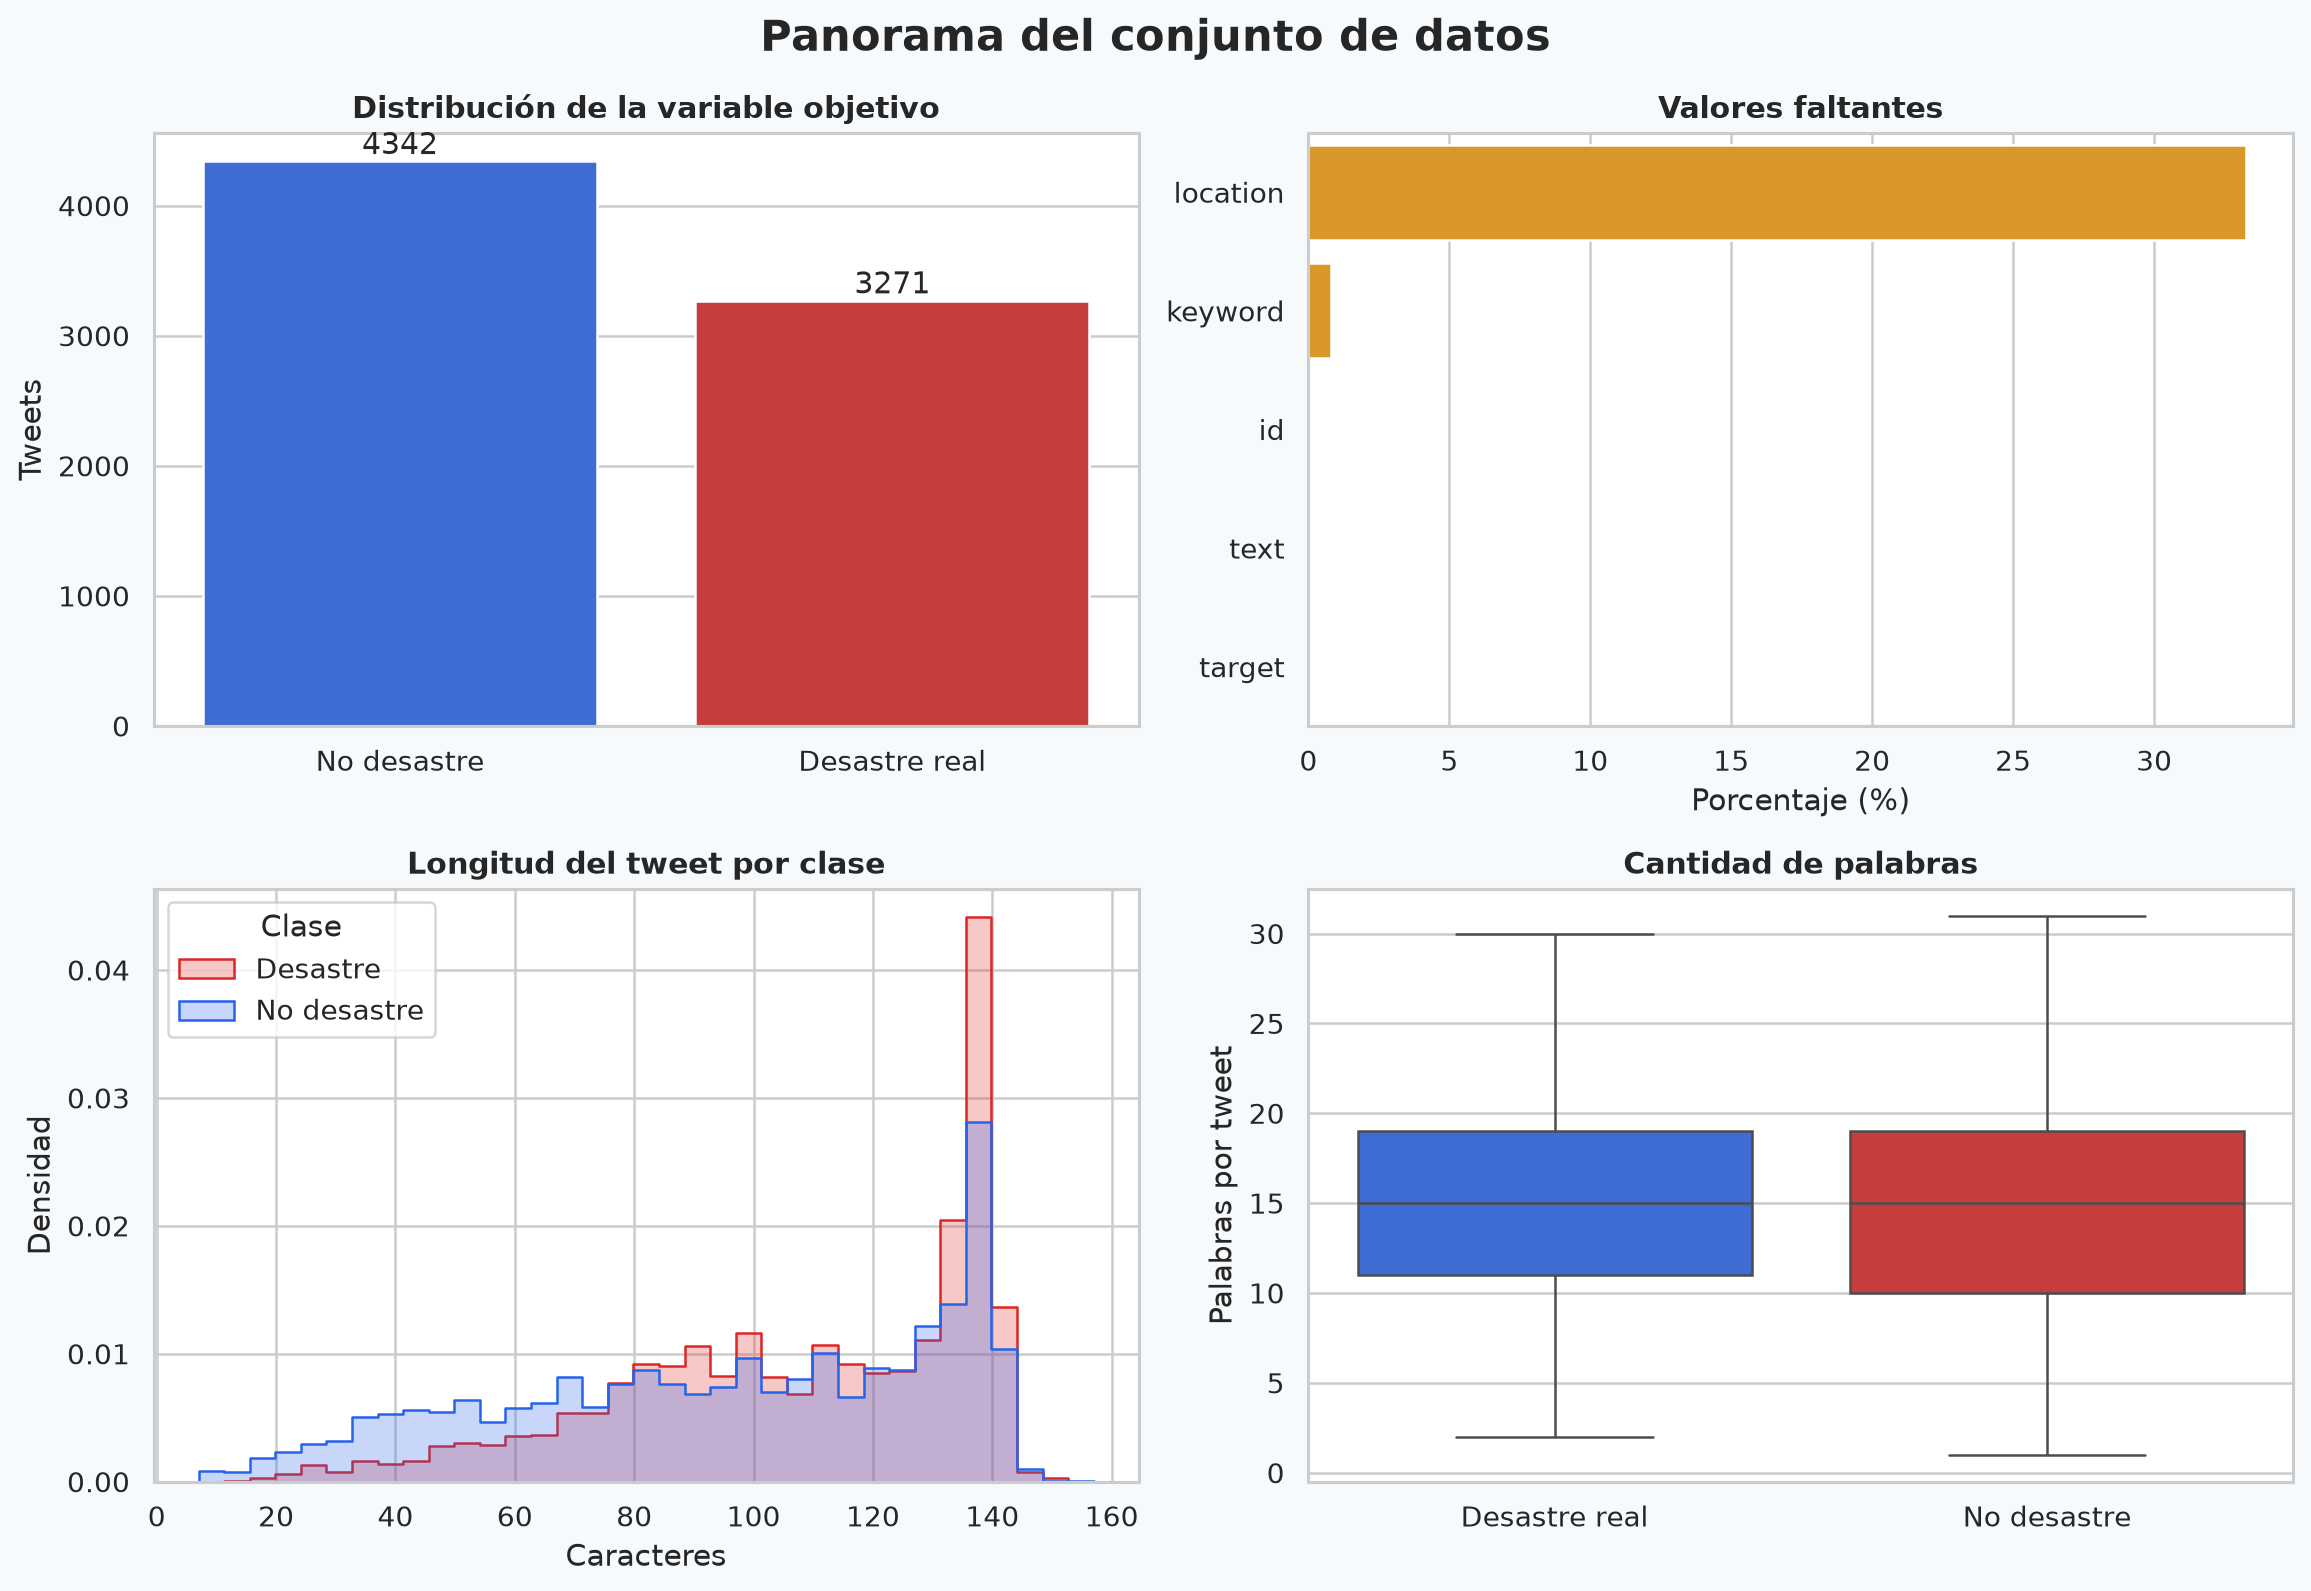
\includegraphics[width=0.96\linewidth]{../outputs/figures/eda_panorama.png}
\caption{Tamaño, balance y longitud del corpus.}
\end{figure}

\begin{figure}[H]
\centering
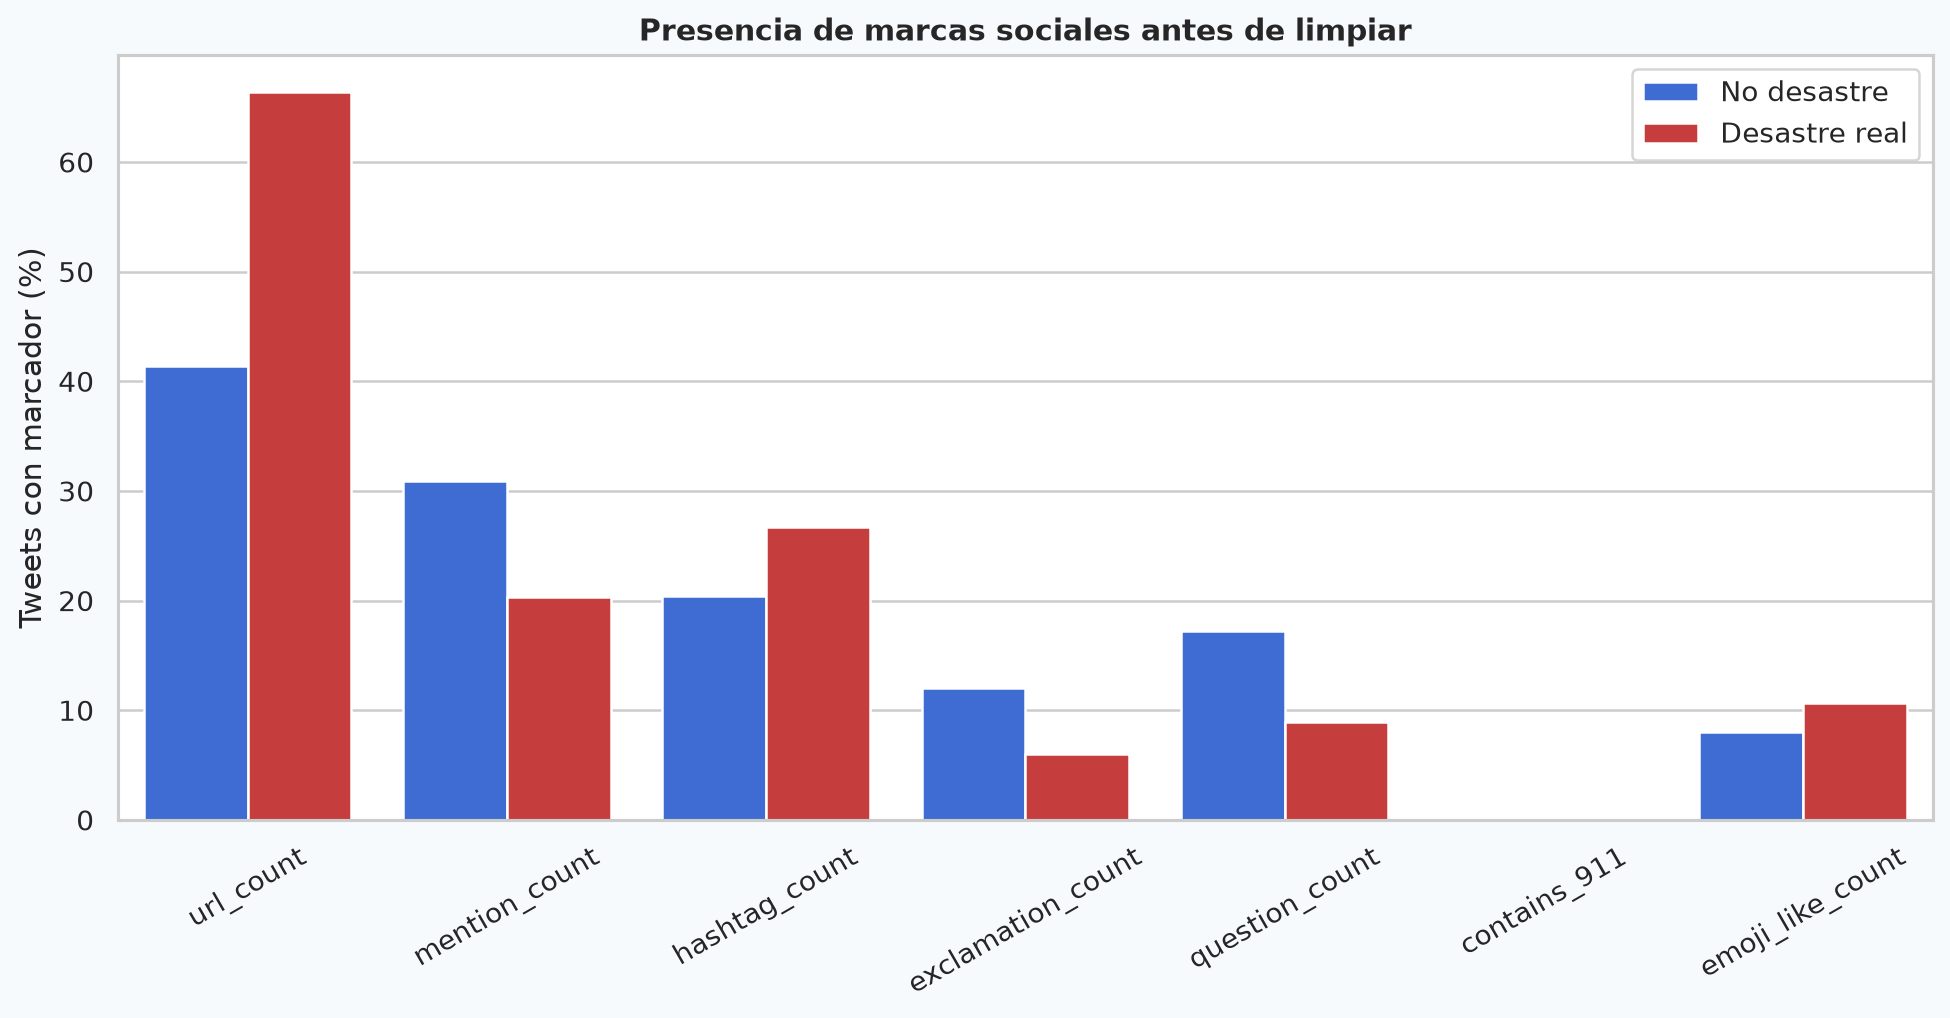
\includegraphics[width=0.96\linewidth]{../outputs/figures/eda_marcadores_sociales.png}
\caption{Marcadores propios de Twitter antes de la limpieza.}
\end{figure}

\section{Preprocesamiento}

Se mantuvieron dos versiones del texto, porque clasificación y sentimiento necesitan información distinta.

\textbf{Texto para clasificación.} Se decodifican entidades HTML, se convierten contracciones como \emph{can't} a \emph{can not}, se eliminan URL y menciones, se retira únicamente el símbolo \# para conservar la palabra del hashtag, se normaliza a minúsculas y se eliminan puntuación, dígitos y stopwords. Las negaciones \emph{no}, \emph{not}, \emph{never} y el token 911 se conservan explícitamente.

\textbf{Texto para sentimiento.} Se aplica limpieza ligera: URL y menciones se retiran, pero se conservan puntuación, emojis y negaciones. Calcular VADER sobre la versión agresivamente depurada destruiría parte de la señal afectiva.

La auditoría automática confirma cero textos originales vacíos, cinco textos limpios vacíos, 3,971 tweets con URL, 2,009 con menciones, 1,761 con hashtag y conservación de los cuatro casos que contienen 911. Los cinco textos vacíos después de limpiar se mantienen como cadenas válidas; TF--IDF los representa como vectores nulos sin perder la correspondencia entre fila y etiqueta.

\section{N-gramas y exploración léxica}

Para un n-grama $g$ y una clase $c$, la probabilidad empírica se definió como:

\[
P(g\mid c)=\frac{f(g,c)}{\sum_{g'}f(g',c)}.
\]

Así, los archivos de resultados distinguen claramente frecuencia bruta y probabilidad. Se calcularon unigramas, bigramas y trigramas por clase. En desastres reales destacan bigramas como \emph{suicide bomber}, \emph{northern california}, \emph{oil spill} y \emph{burning buildings}; aportan un contexto más específico que palabras aisladas.

\begin{figure}[H]
\centering
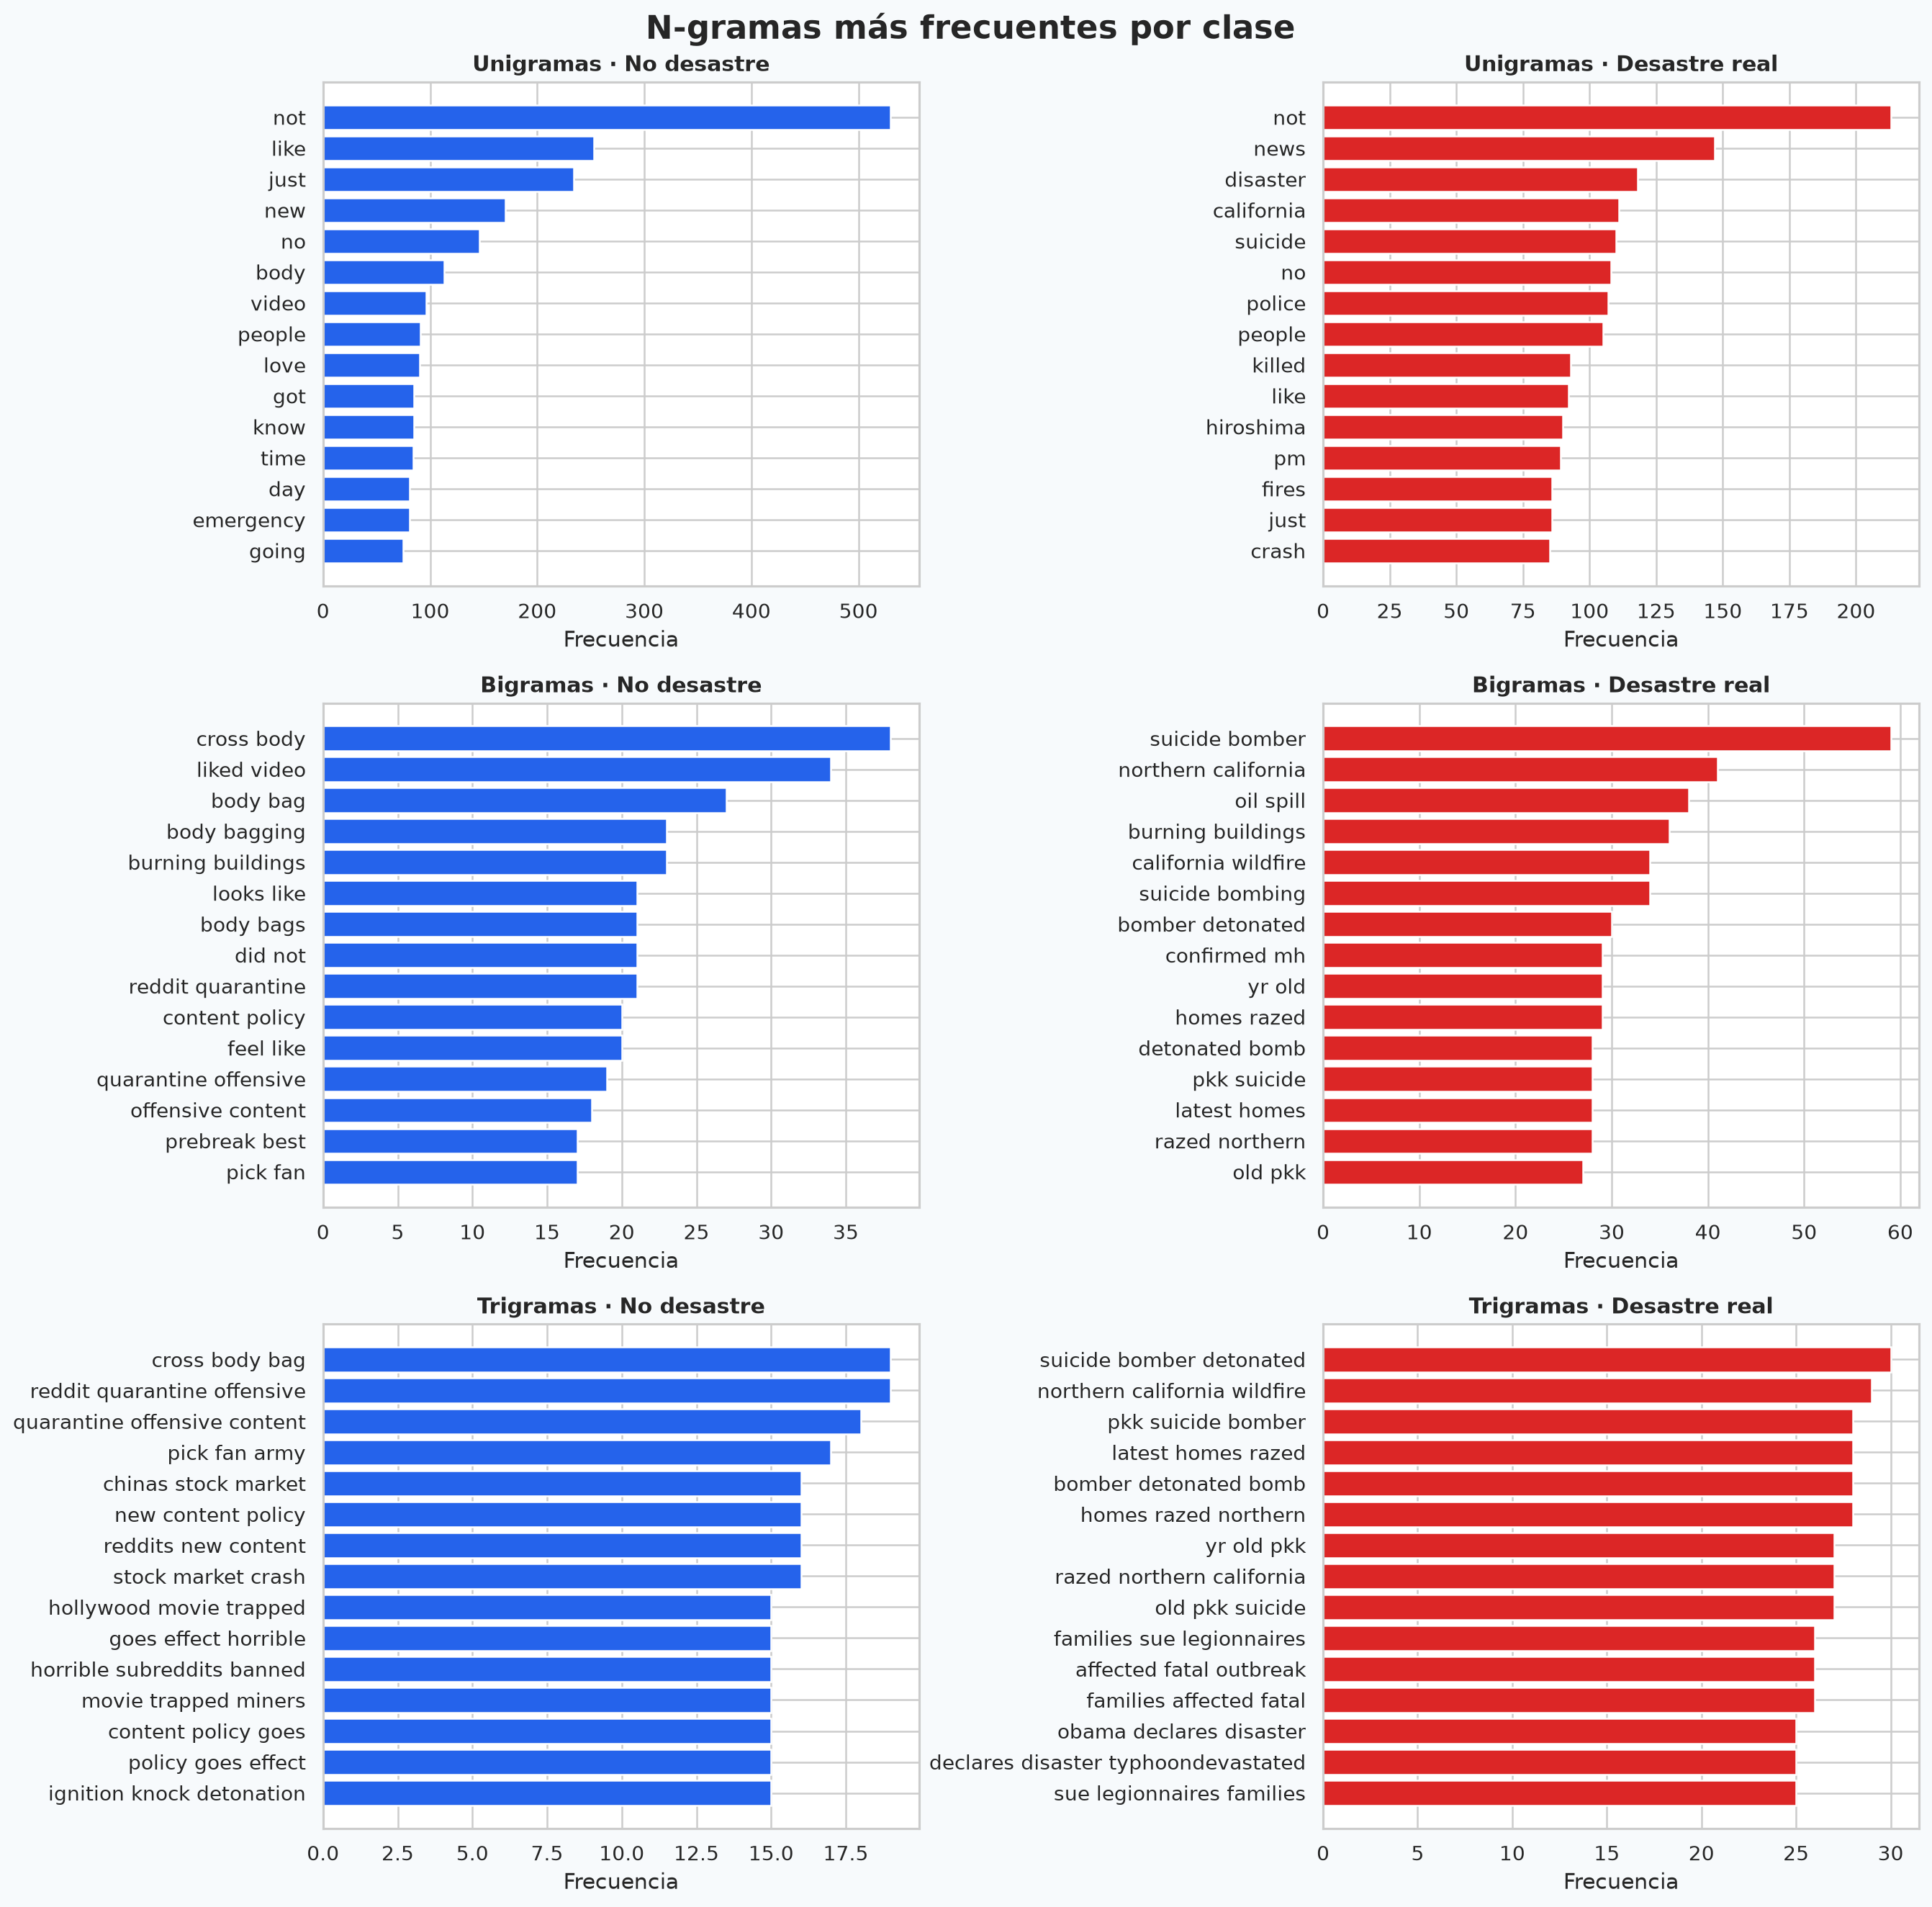
\includegraphics[width=0.98\linewidth]{../outputs/figures/ngramas_por_clase.png}
\caption{N-gramas principales por clase y orden.}
\end{figure}

Para reducir el sesgo hacia términos globalmente frecuentes se añadió un cociente logarítmico suavizado. Valores positivos identifican vocabulario proporcionalmente más asociado con desastres y valores negativos, vocabulario más característico de la clase contraria.

\begin{figure}[H]
\centering
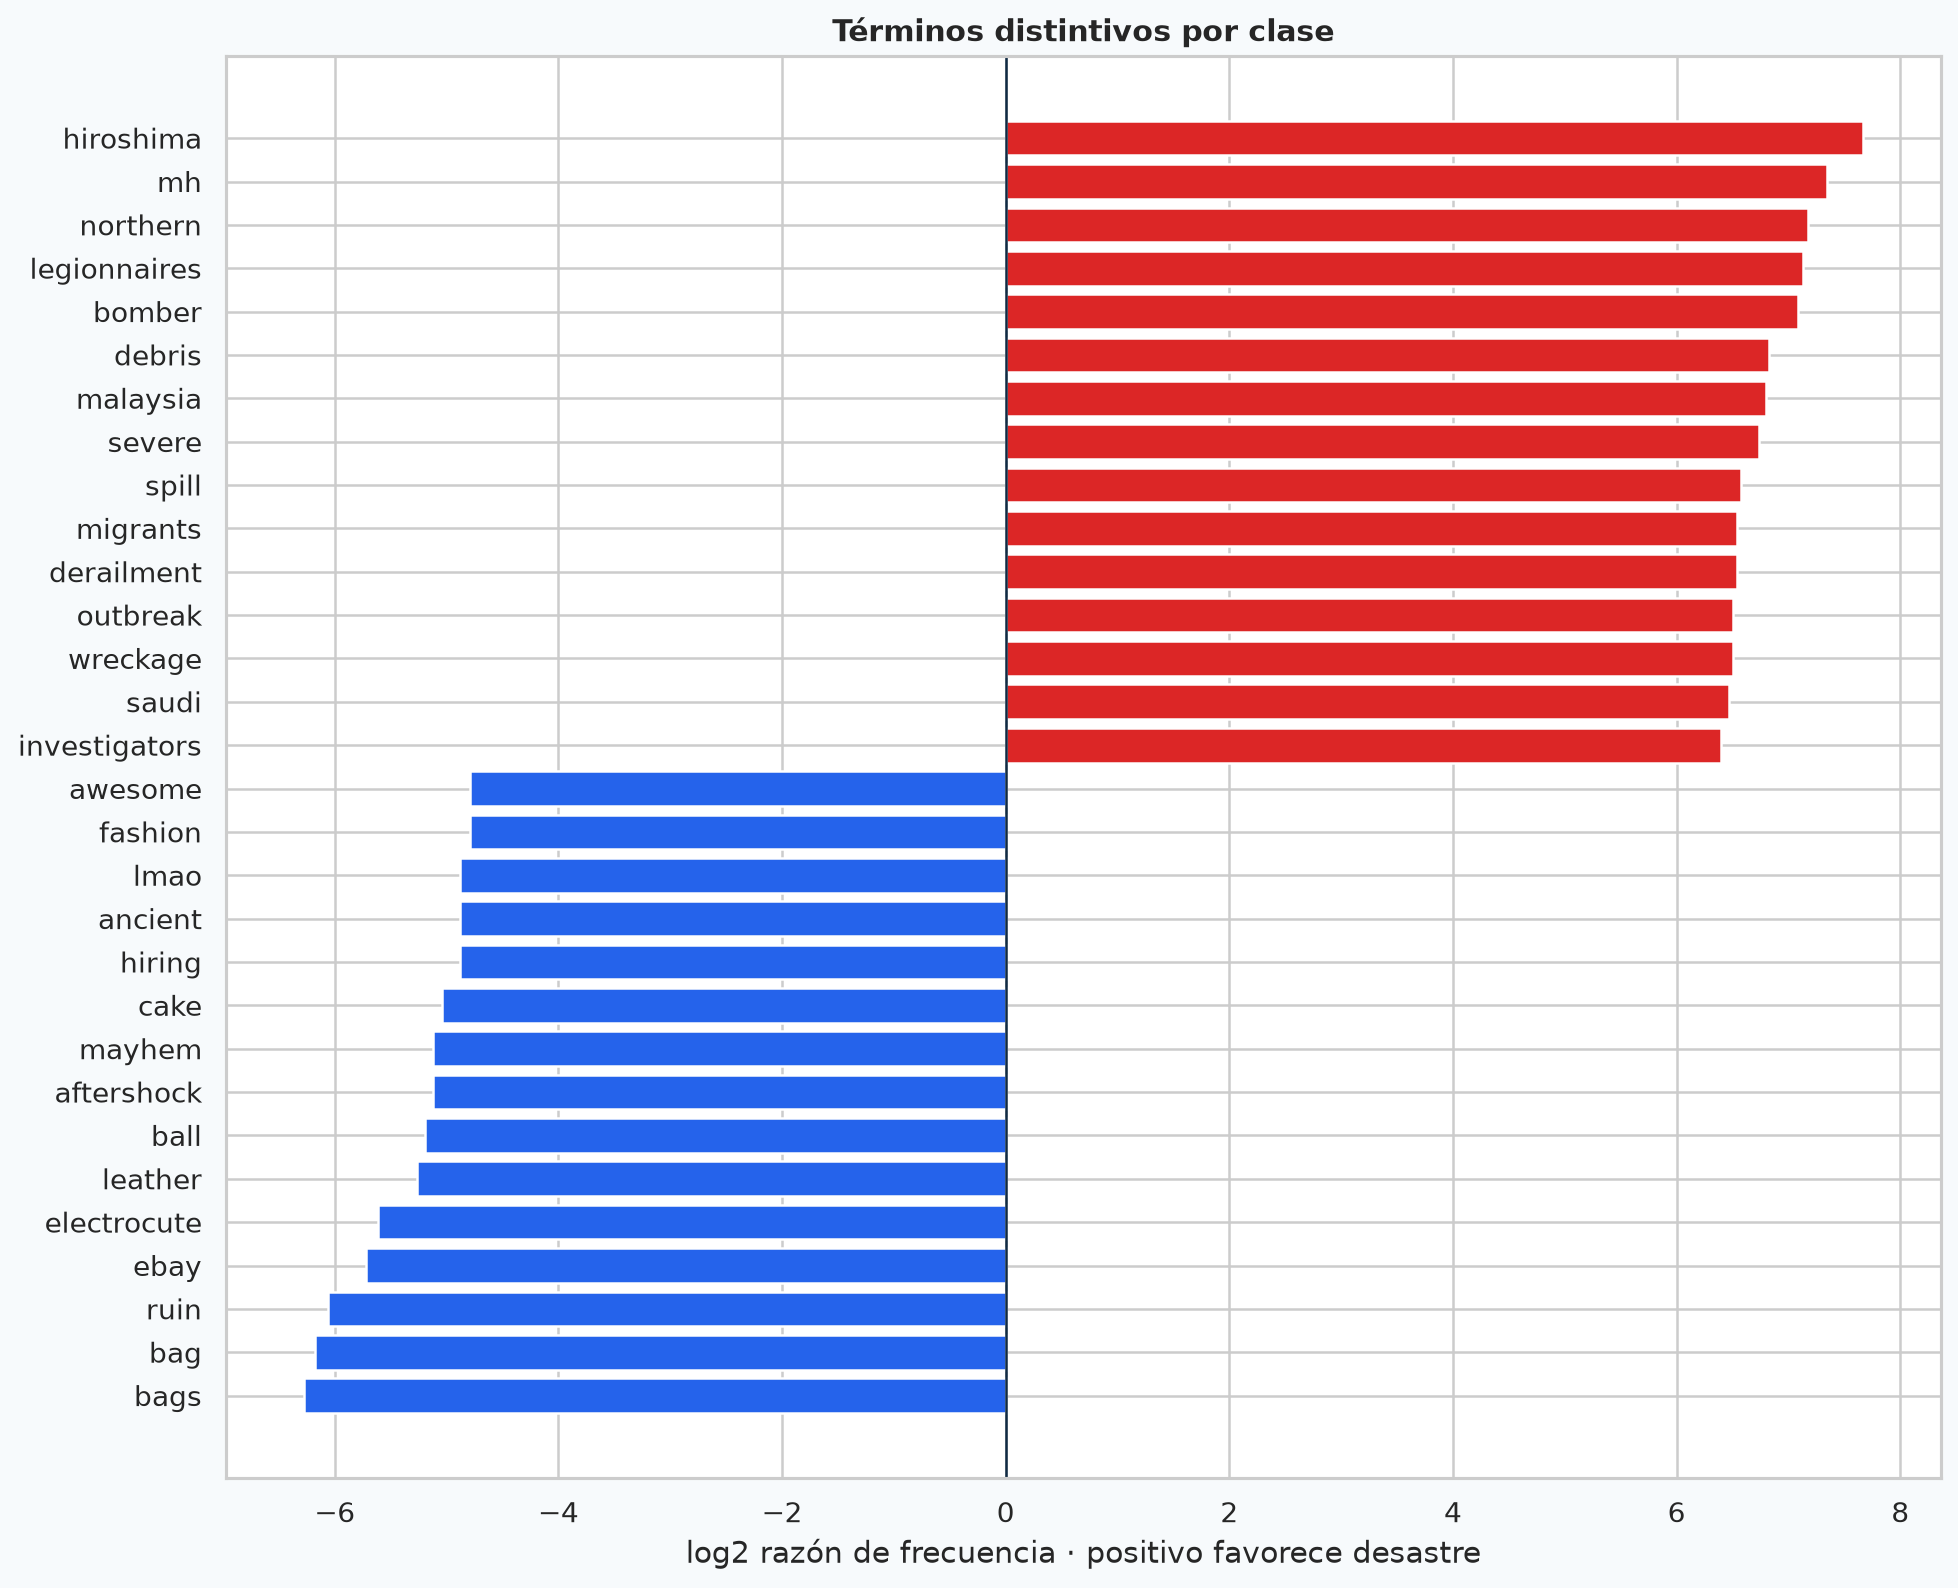
\includegraphics[width=0.90\linewidth]{../outputs/figures/unigramas_distintivos.png}
\caption{Vocabulario distintivo según cociente logarítmico suavizado.}
\end{figure}

\section{Modelado preliminar}

\subsection{Diseño experimental}

Se realizó una única división estratificada con 80\% para entrenamiento (6,090 filas) y 20\% para validación (1,523 filas), usando semilla 42. Todos los modelos recibieron exactamente los mismos ejemplos. La representación TF--IDF usa unigramas y bigramas, frecuencia mínima de dos, frecuencia máxima de 98\%, escalamiento sublineal y un máximo de 35,000 características.

Se compararon cuatro alternativas: baseline de clase mayoritaria, Naive Bayes complementario, regresión logística con ponderación de clases y SVM lineal calibrado. La calibración permite interpretar la salida del SVM como probabilidad aproximada y calcular ROC--AUC.

\begin{table}[H]
\centering
\caption{Resultados sobre el conjunto de validación.}
\small
\begin{tabular}{lrrrrrr}
\toprule
Modelo & Acc. & Prec. & Recall & F1 & F1 macro & AUC \\
\midrule
Regresión logística & \textbf{0.813} & 0.785 & \textbf{0.777} & \textbf{0.781} & \textbf{0.809} & \textbf{0.867} \\
SVM calibrado & 0.810 & \textbf{0.807} & 0.731 & 0.767 & 0.803 & 0.861 \\
Naive Bayes compl. & 0.807 & 0.800 & 0.734 & 0.766 & 0.801 & 0.864 \\
Baseline mayoritario & 0.571 & 0.000 & 0.000 & 0.000 & 0.363 & 0.500 \\
\bottomrule
\end{tabular}
\end{table}

\begin{figure}[H]
\centering
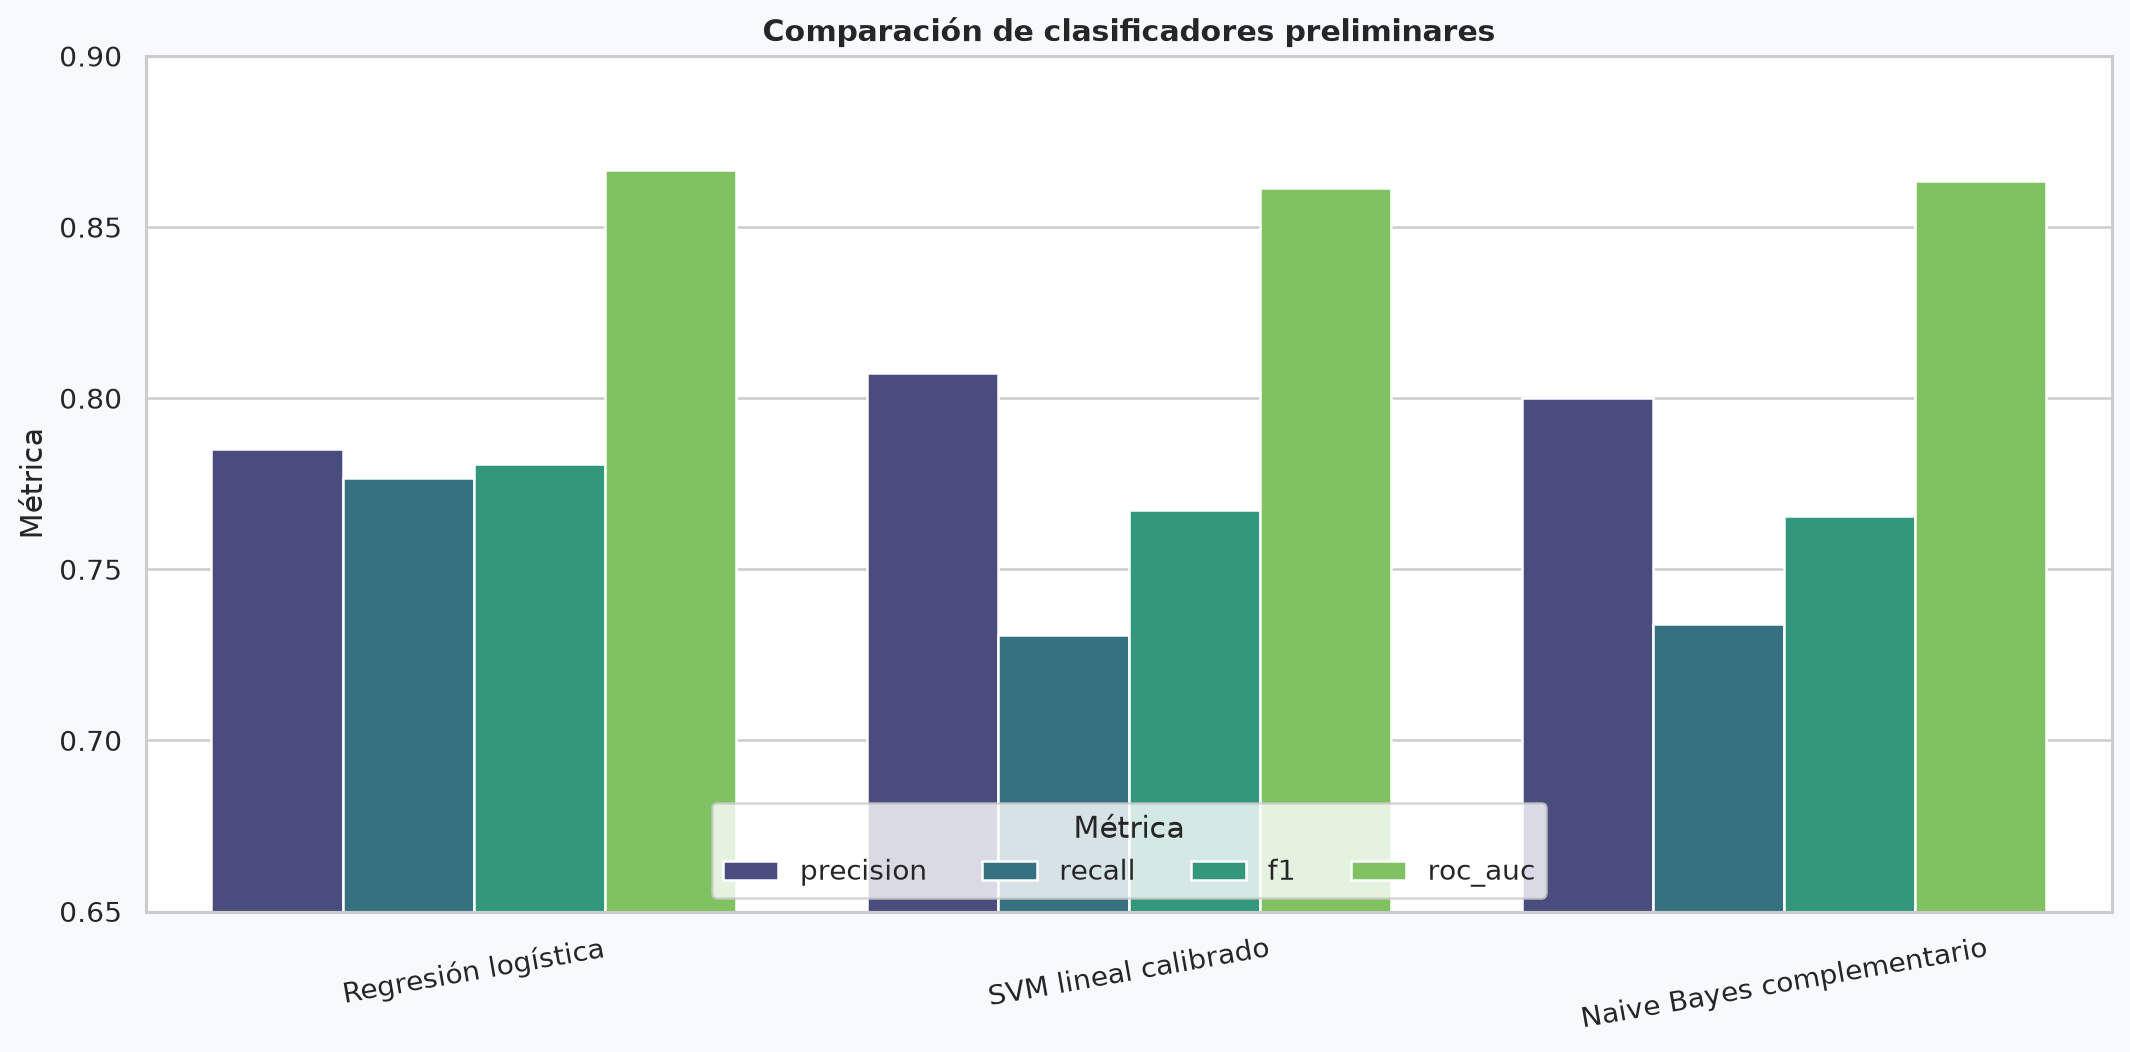
\includegraphics[width=0.96\linewidth]{../outputs/figures/modelos_comparacion.png}
\caption{Comparación de métricas de los modelos preliminares.}
\end{figure}

\subsection{Errores e interpretación}

La regresión logística clasifica correctamente 730 no desastres y 508 desastres. Produce 139 falsos positivos y 146 falsos negativos. El SVM reduce los falsos positivos a 114, pero aumenta los falsos negativos a 176. Dado que omitir una emergencia puede ser más costoso que emitir una alerta falsa, el mayor recall de la regresión logística favorece su selección preliminar.

\begin{figure}[H]
\centering
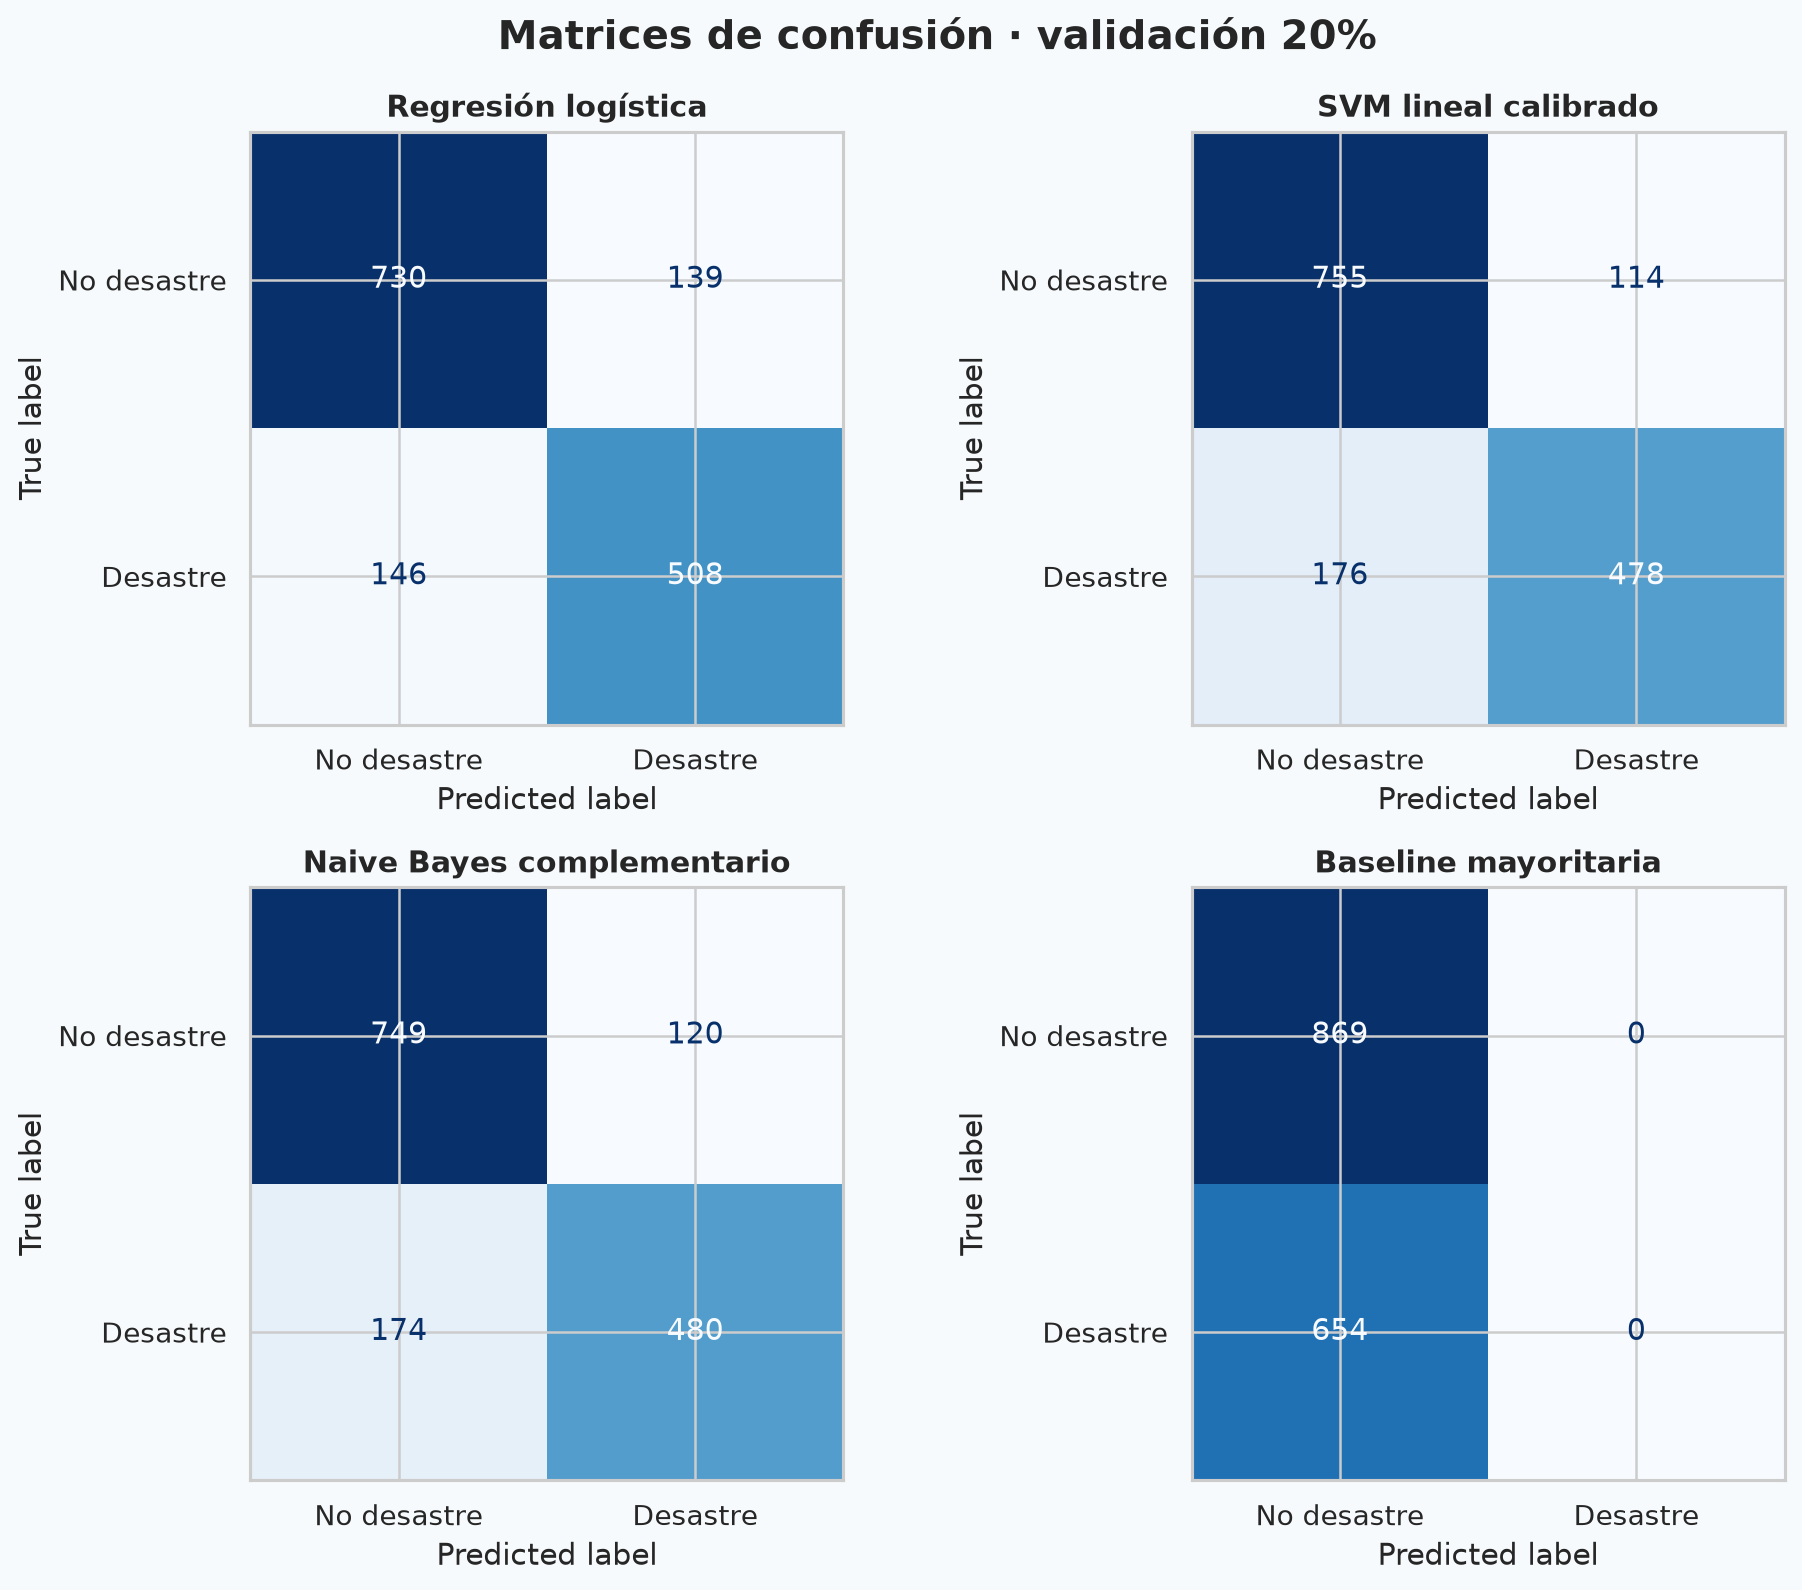
\includegraphics[width=0.98\linewidth]{../outputs/figures/modelos_matrices_confusion.png}
\caption{Matrices de confusión sobre una partición común.}
\end{figure}

\begin{figure}[H]
\centering
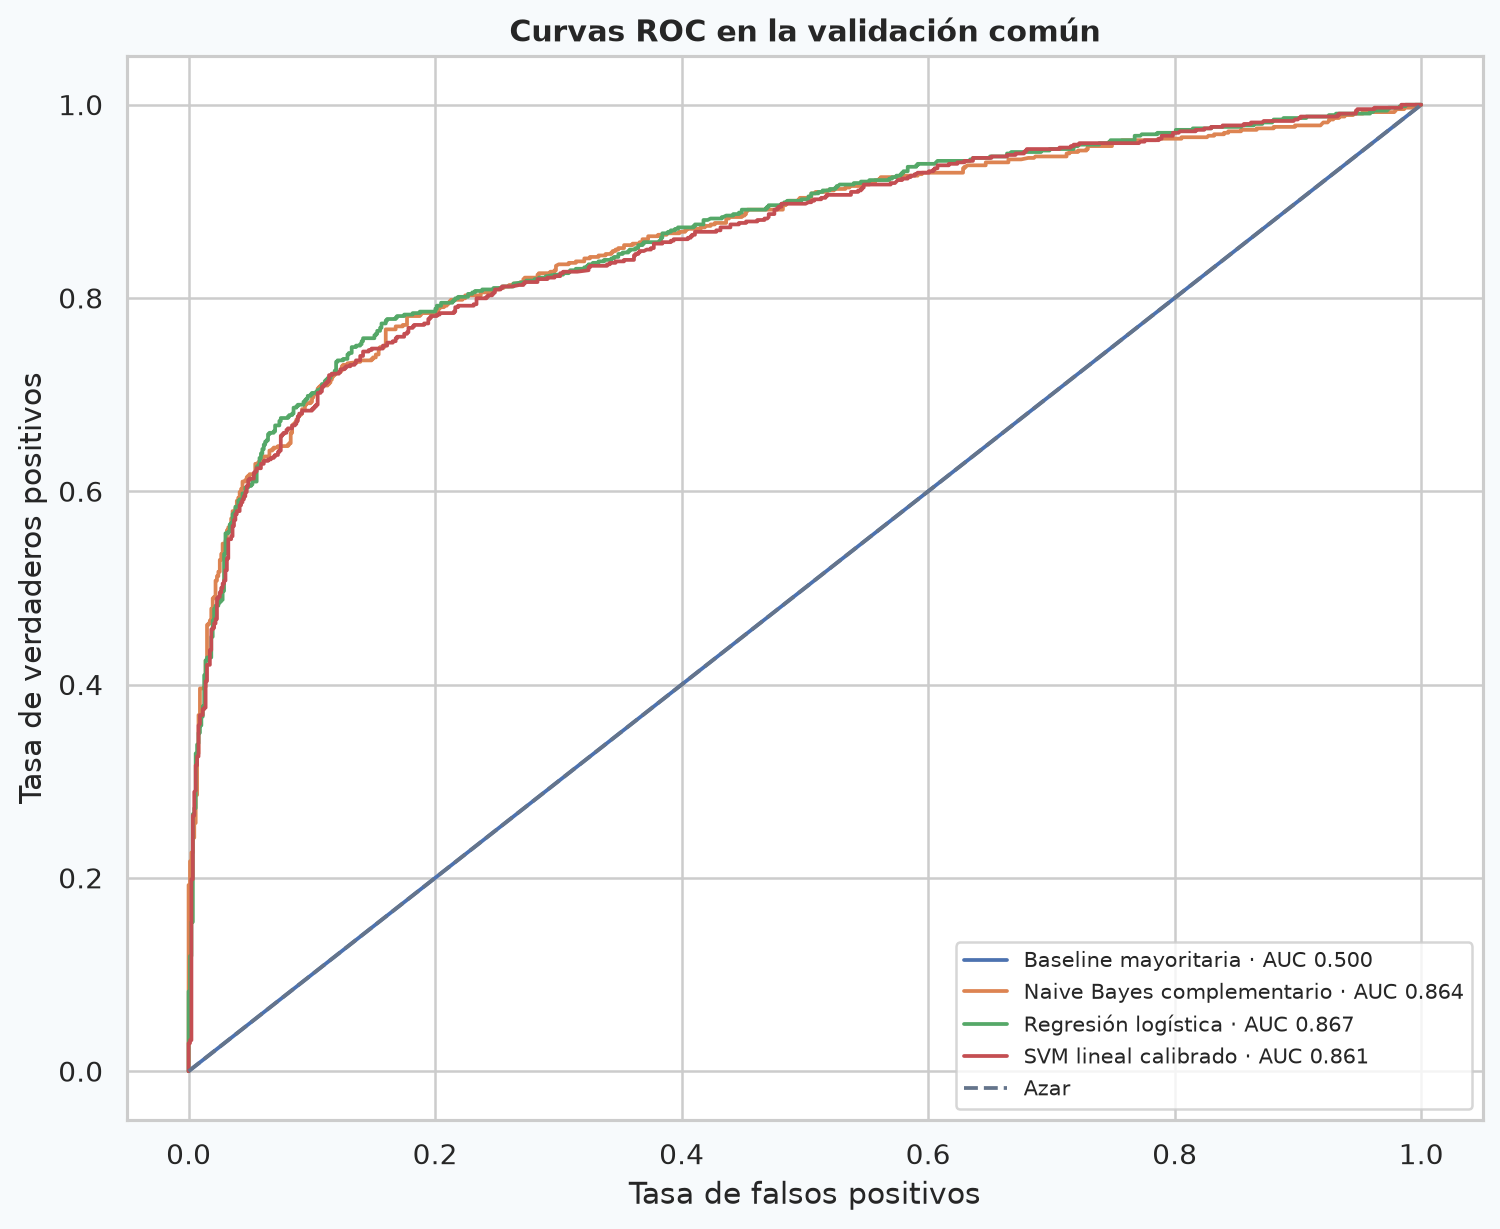
\includegraphics[width=0.78\linewidth]{../outputs/figures/modelos_curvas_roc.png}
\caption{Curvas ROC de los clasificadores probabilísticos.}
\end{figure}

\section{Función de inferencia}

La función \texttt{predict\_tweet} acepta texto sin preprocesar, llama a la misma rutina de limpieza utilizada para entrenar, calcula la probabilidad de desastre y entrega una clase legible. Si se proporciona el analizador VADER, añade etiqueta y polaridad de sentimiento. El script \texttt{scripts/predict\_tweet.py} expone esa función desde la terminal.

En los ejemplos de control, una evacuación por incendio obtuvo probabilidad 0.877 de desastre y una inundación reportada por servicios de emergencia, 0.753. La frase que describe una película como ``total disaster'' obtuvo 0.353 y se clasificó como no desastre. Este último caso ilustra que el modelo aprovecha el contexto y no una sola palabra clave.

\section{Sentimiento exploratorio}

Se aplicó VADER al texto con limpieza ligera. La polaridad media fue -0.052 para no desastres y -0.266 para desastres reales; las medianas fueron 0.000 y -0.318, respectivamente. La diferencia descriptiva es coherente con la hipótesis de que los reportes reales tienden a ser más negativos, pero todavía no prueba significancia ni utilidad predictiva incremental.

\begin{figure}[H]
\centering
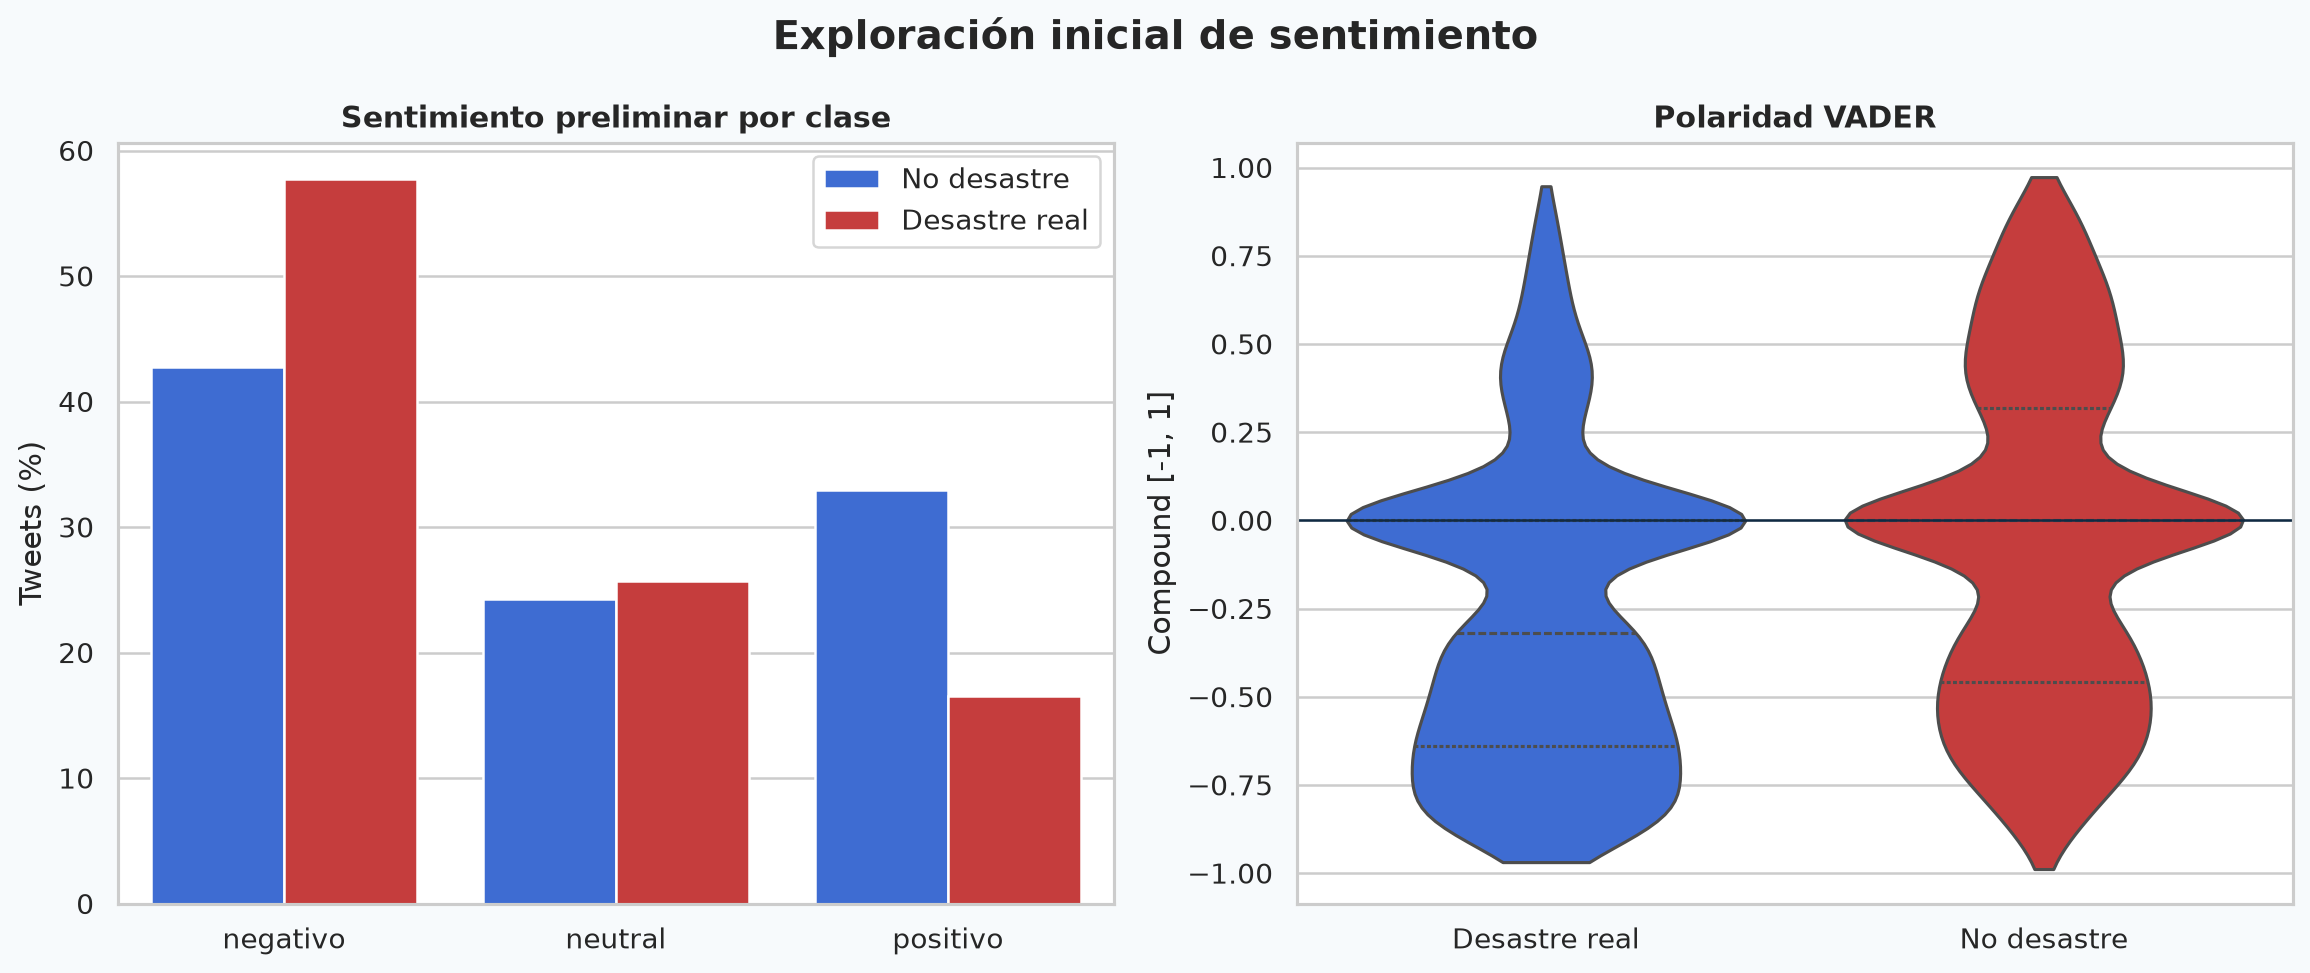
\includegraphics[width=0.96\linewidth]{../outputs/figures/sentimiento_exploratorio.png}
\caption{Distribución descriptiva del sentimiento por clase.}
\end{figure}

\section{Reproducibilidad y controles de calidad}

El proyecto incluye dependencias en \texttt{pyproject.toml}, archivo \texttt{requirements.txt}, módulos separados para análisis, preprocesamiento, modelado y sentimiento, y scripts de ejecución. Nueve pruebas verifican el esquema del conjunto, blancos de clase válidos, normalización de probabilidades, extracción de atributos, conservación de negaciones y 911, limpieza ligera para sentimiento, disponibilidad de los modelos y contrato de la función predictiva.

Los datos derivados se almacenan comprimidos, las figuras y tablas se regeneran con un comando y el notebook se entrega ejecutado sin errores. Las credenciales no forman parte del repositorio.

\section{Estado frente a la guía}

\begin{table}[H]
\centering
\caption{Cobertura del avance y reserva para la entrega final.}
\begin{tabularx}{\linewidth}{>{\raggedright\arraybackslash}X l}
\toprule
Componente & Estado \\
\midrule
Descripción, limpieza y EDA & Completo \\
Unigramas, bigramas y trigramas con probabilidades & Completo \\
Modelos preliminares y métricas & Completo \\
Función para tweets nuevos & Completo \\
Sentimiento & Preliminar \\
Top 10 positivo y negativo con interpretación & Pendiente final \\
Contraste estadístico por clase & Pendiente final \\
Variable de negatividad y reentrenamiento & Pendiente final \\
Afinación, errores y conclusiones definitivas & Pendiente final \\
\bottomrule
\end{tabularx}
\end{table}

\section{Conclusiones provisionales}

El corpus ofrece señal suficiente para separar el uso literal y figurado del lenguaje de desastres. La regresión logística proporciona el mejor equilibrio preliminar y supera ampliamente el baseline. La conservación de contexto mediante bigramas, negaciones y hashtags es metodológicamente importante, mientras que la separación entre limpieza de clasificación y sentimiento evita perder señales afectivas.

El 25\% final se concentrará en seleccionar e interpretar los diez tweets más positivos y negativos, contrastar formalmente el sentimiento entre clases, incorporar una variable de negatividad y repetir la evaluación bajo el mismo protocolo. Solo después de esos pasos se formularán conclusiones definitivas sobre el aporte del sentimiento y el modelo final.

\end{document}
